\chapter{Módulo 5: Motores de Corriente Continua}

\section{Paso 1:}

Instalar capacitor cerámico 0.1uF C12

\begin{figure}[h]
	\centering
	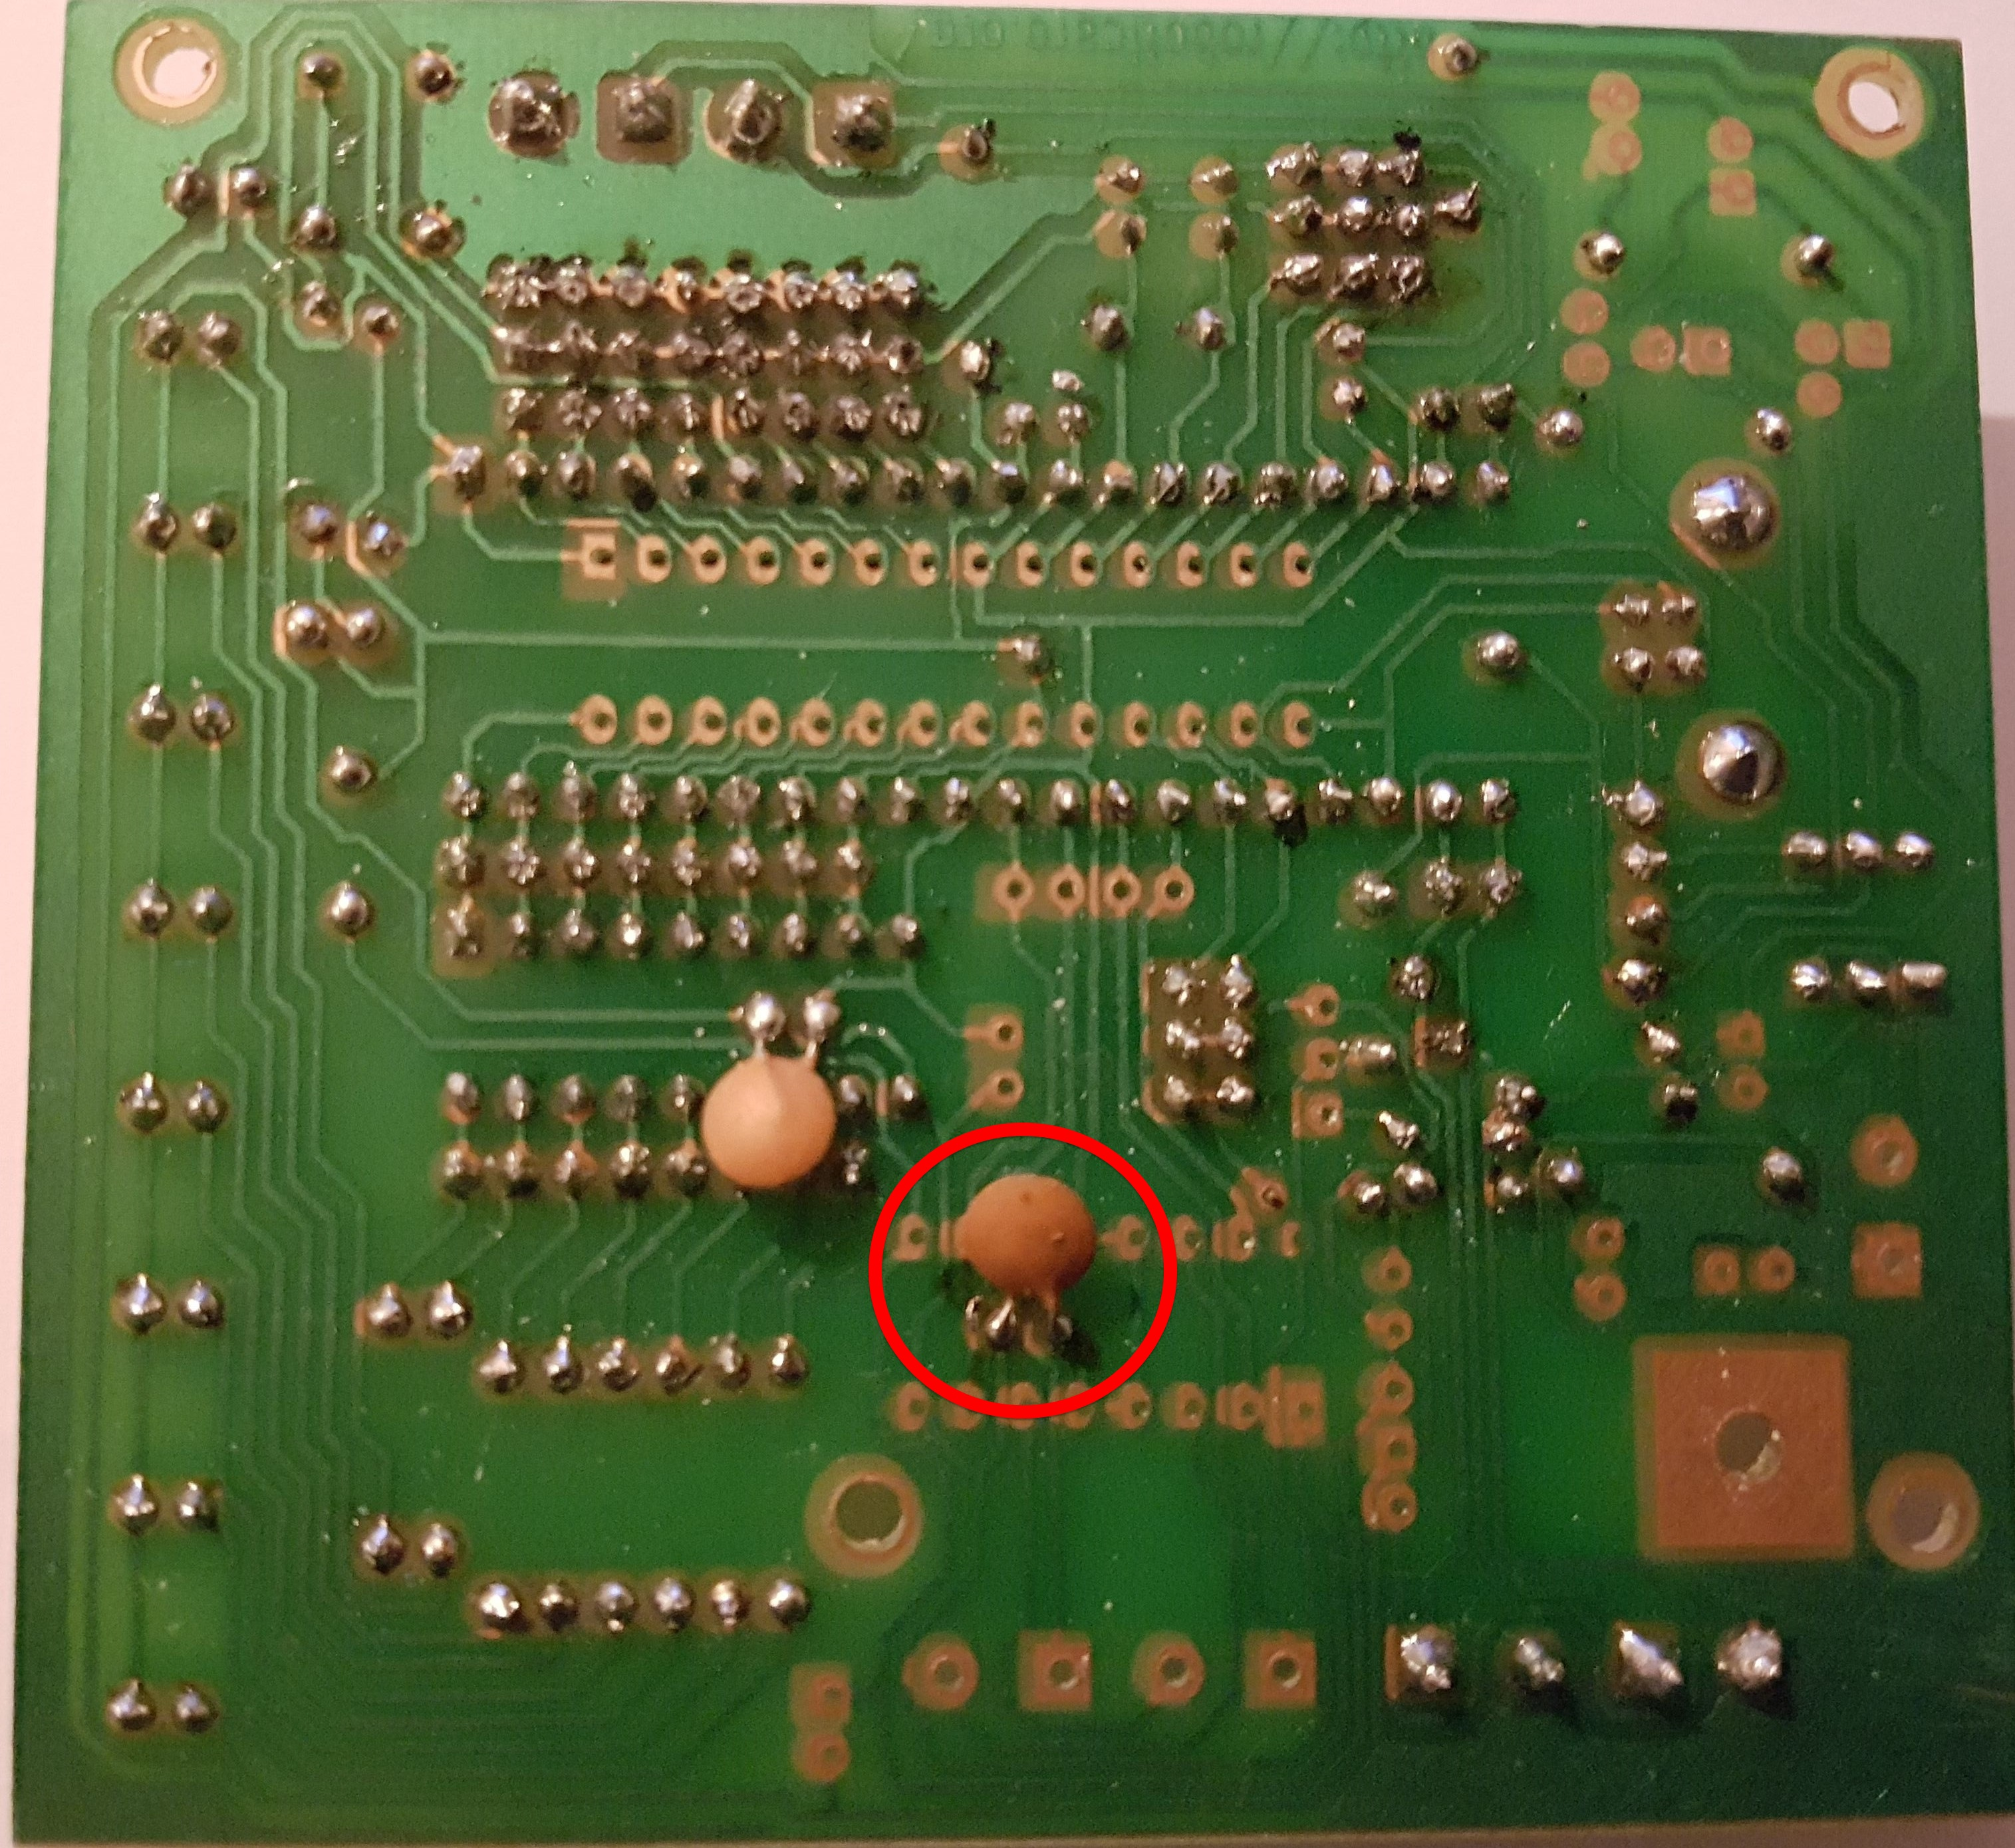
\includegraphics[width=0.8\linewidth]{Modulo_5/M5_1}
	\caption{Módulo 5 - Paso 1}
	\label{fig:M5_1}
\end{figure}

\newpage

\section{Paso 2:}

Instalar zócalo de 16 patas (2x8) U3 Tomar en cuenta alinear la muesca del diagrama de la placa con la muesca del zócalo.

\begin{figure}[h]
	\centering
	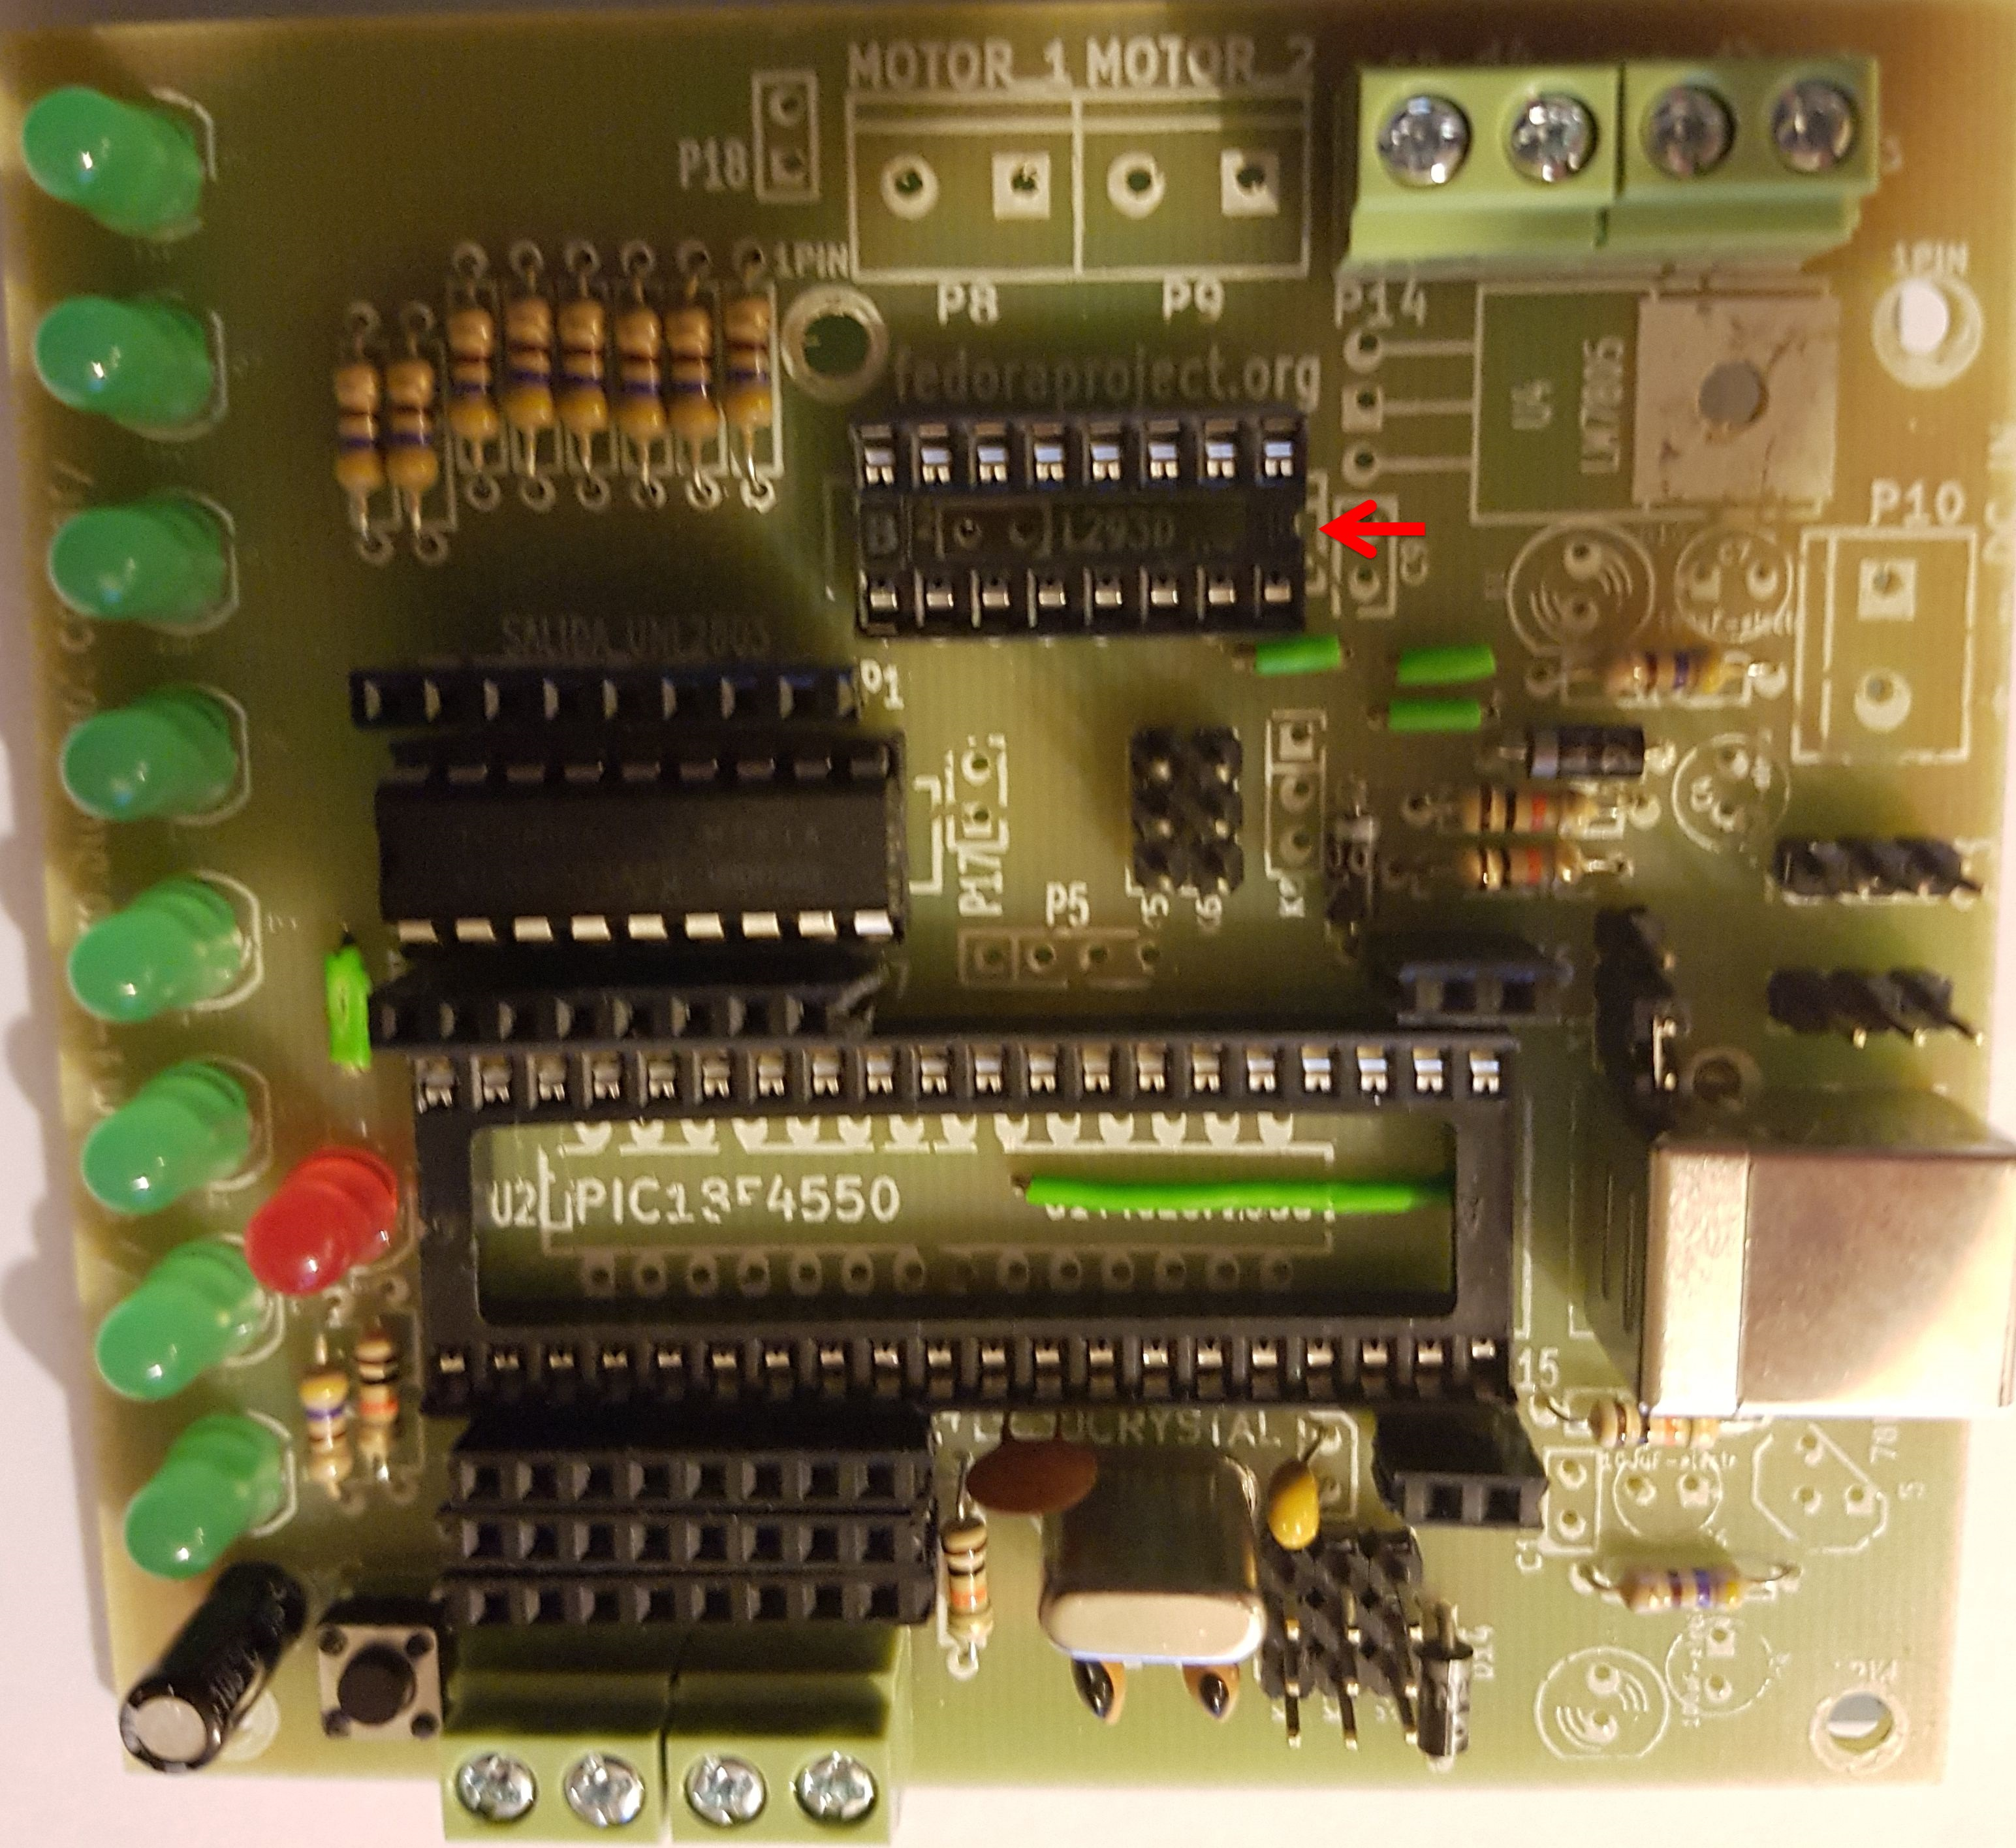
\includegraphics[width=0.8\linewidth]{Modulo_5/M5_2}
	\caption{Módulo 5 - Paso 2}
	\label{fig:M5_2}
\end{figure}

\newpage

\section{Paso 3:}

Instalar pines hembras P5 (Estos pines pueden usarse para tomar la señal que va al puente H)

\begin{figure}[h]
	\centering
	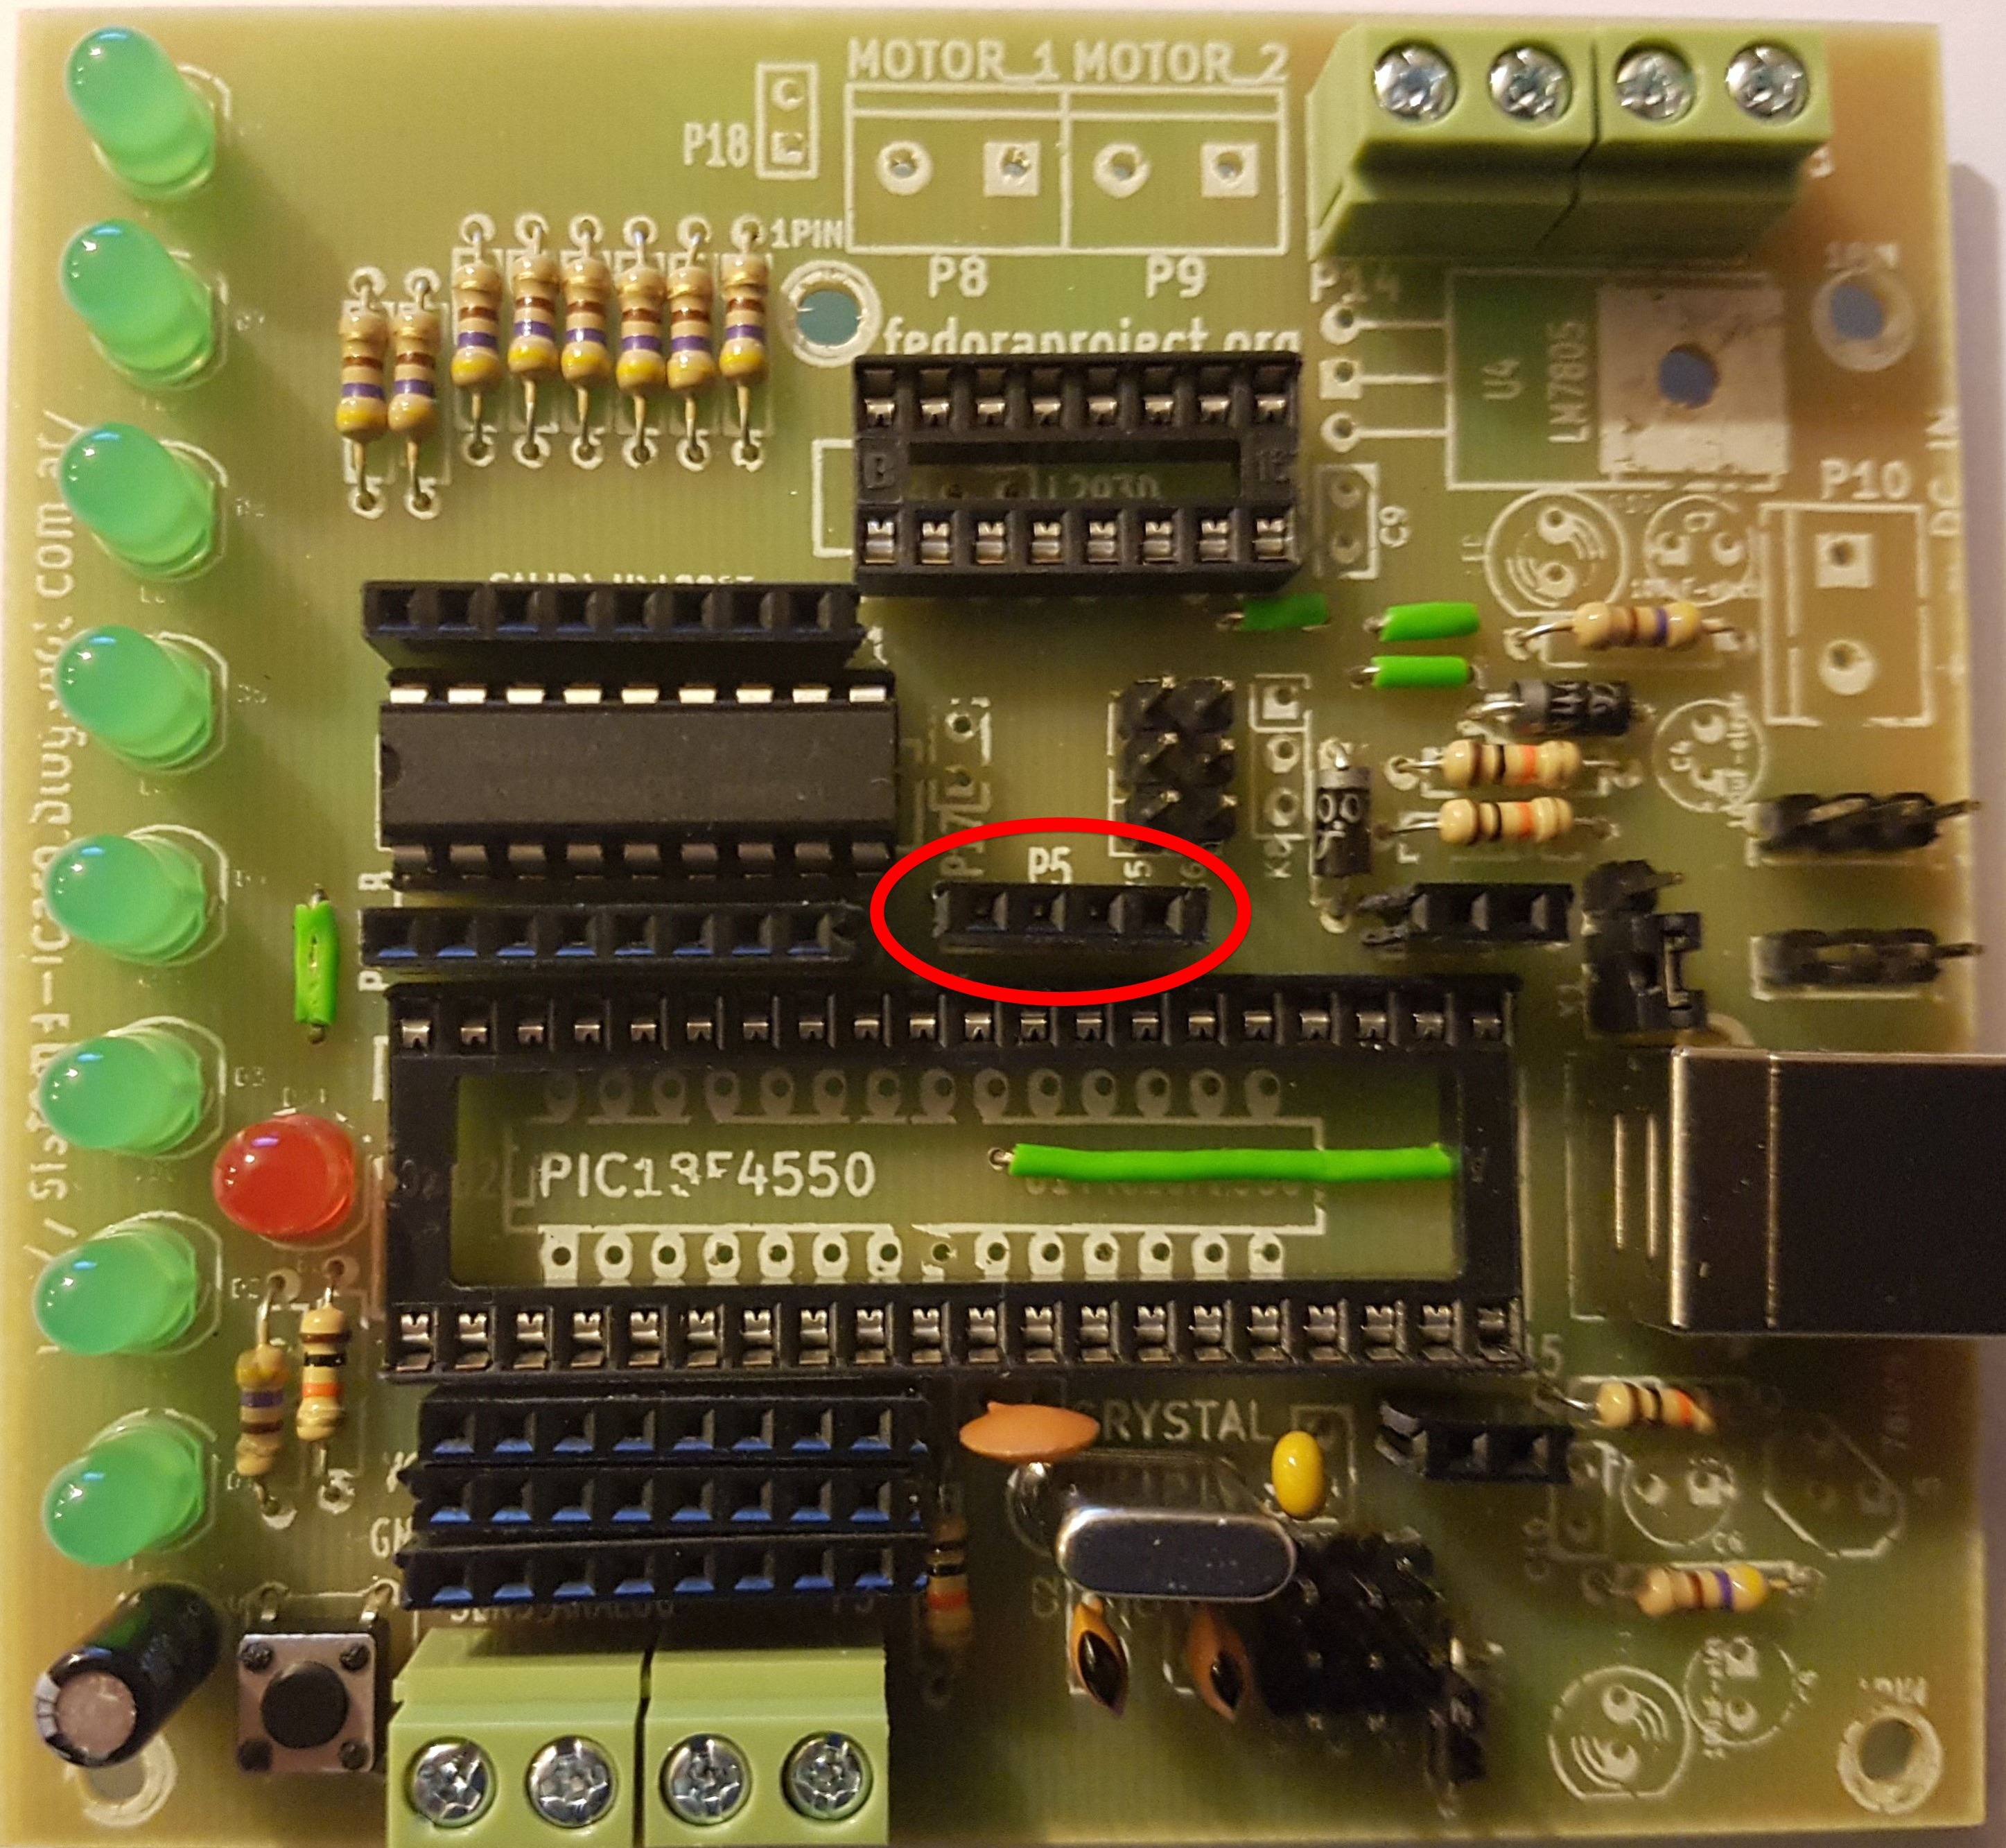
\includegraphics[width=0.8\linewidth]{Modulo_5/M5_3}
	\caption{Módulo 5 - Paso 3}
	\label{fig:M5_3}
\end{figure}

\newpage

\section{Paso 4:}

Instalar borneras de dos posiciones de motores. P8 y P9

\begin{figure}[h]
	\centering
	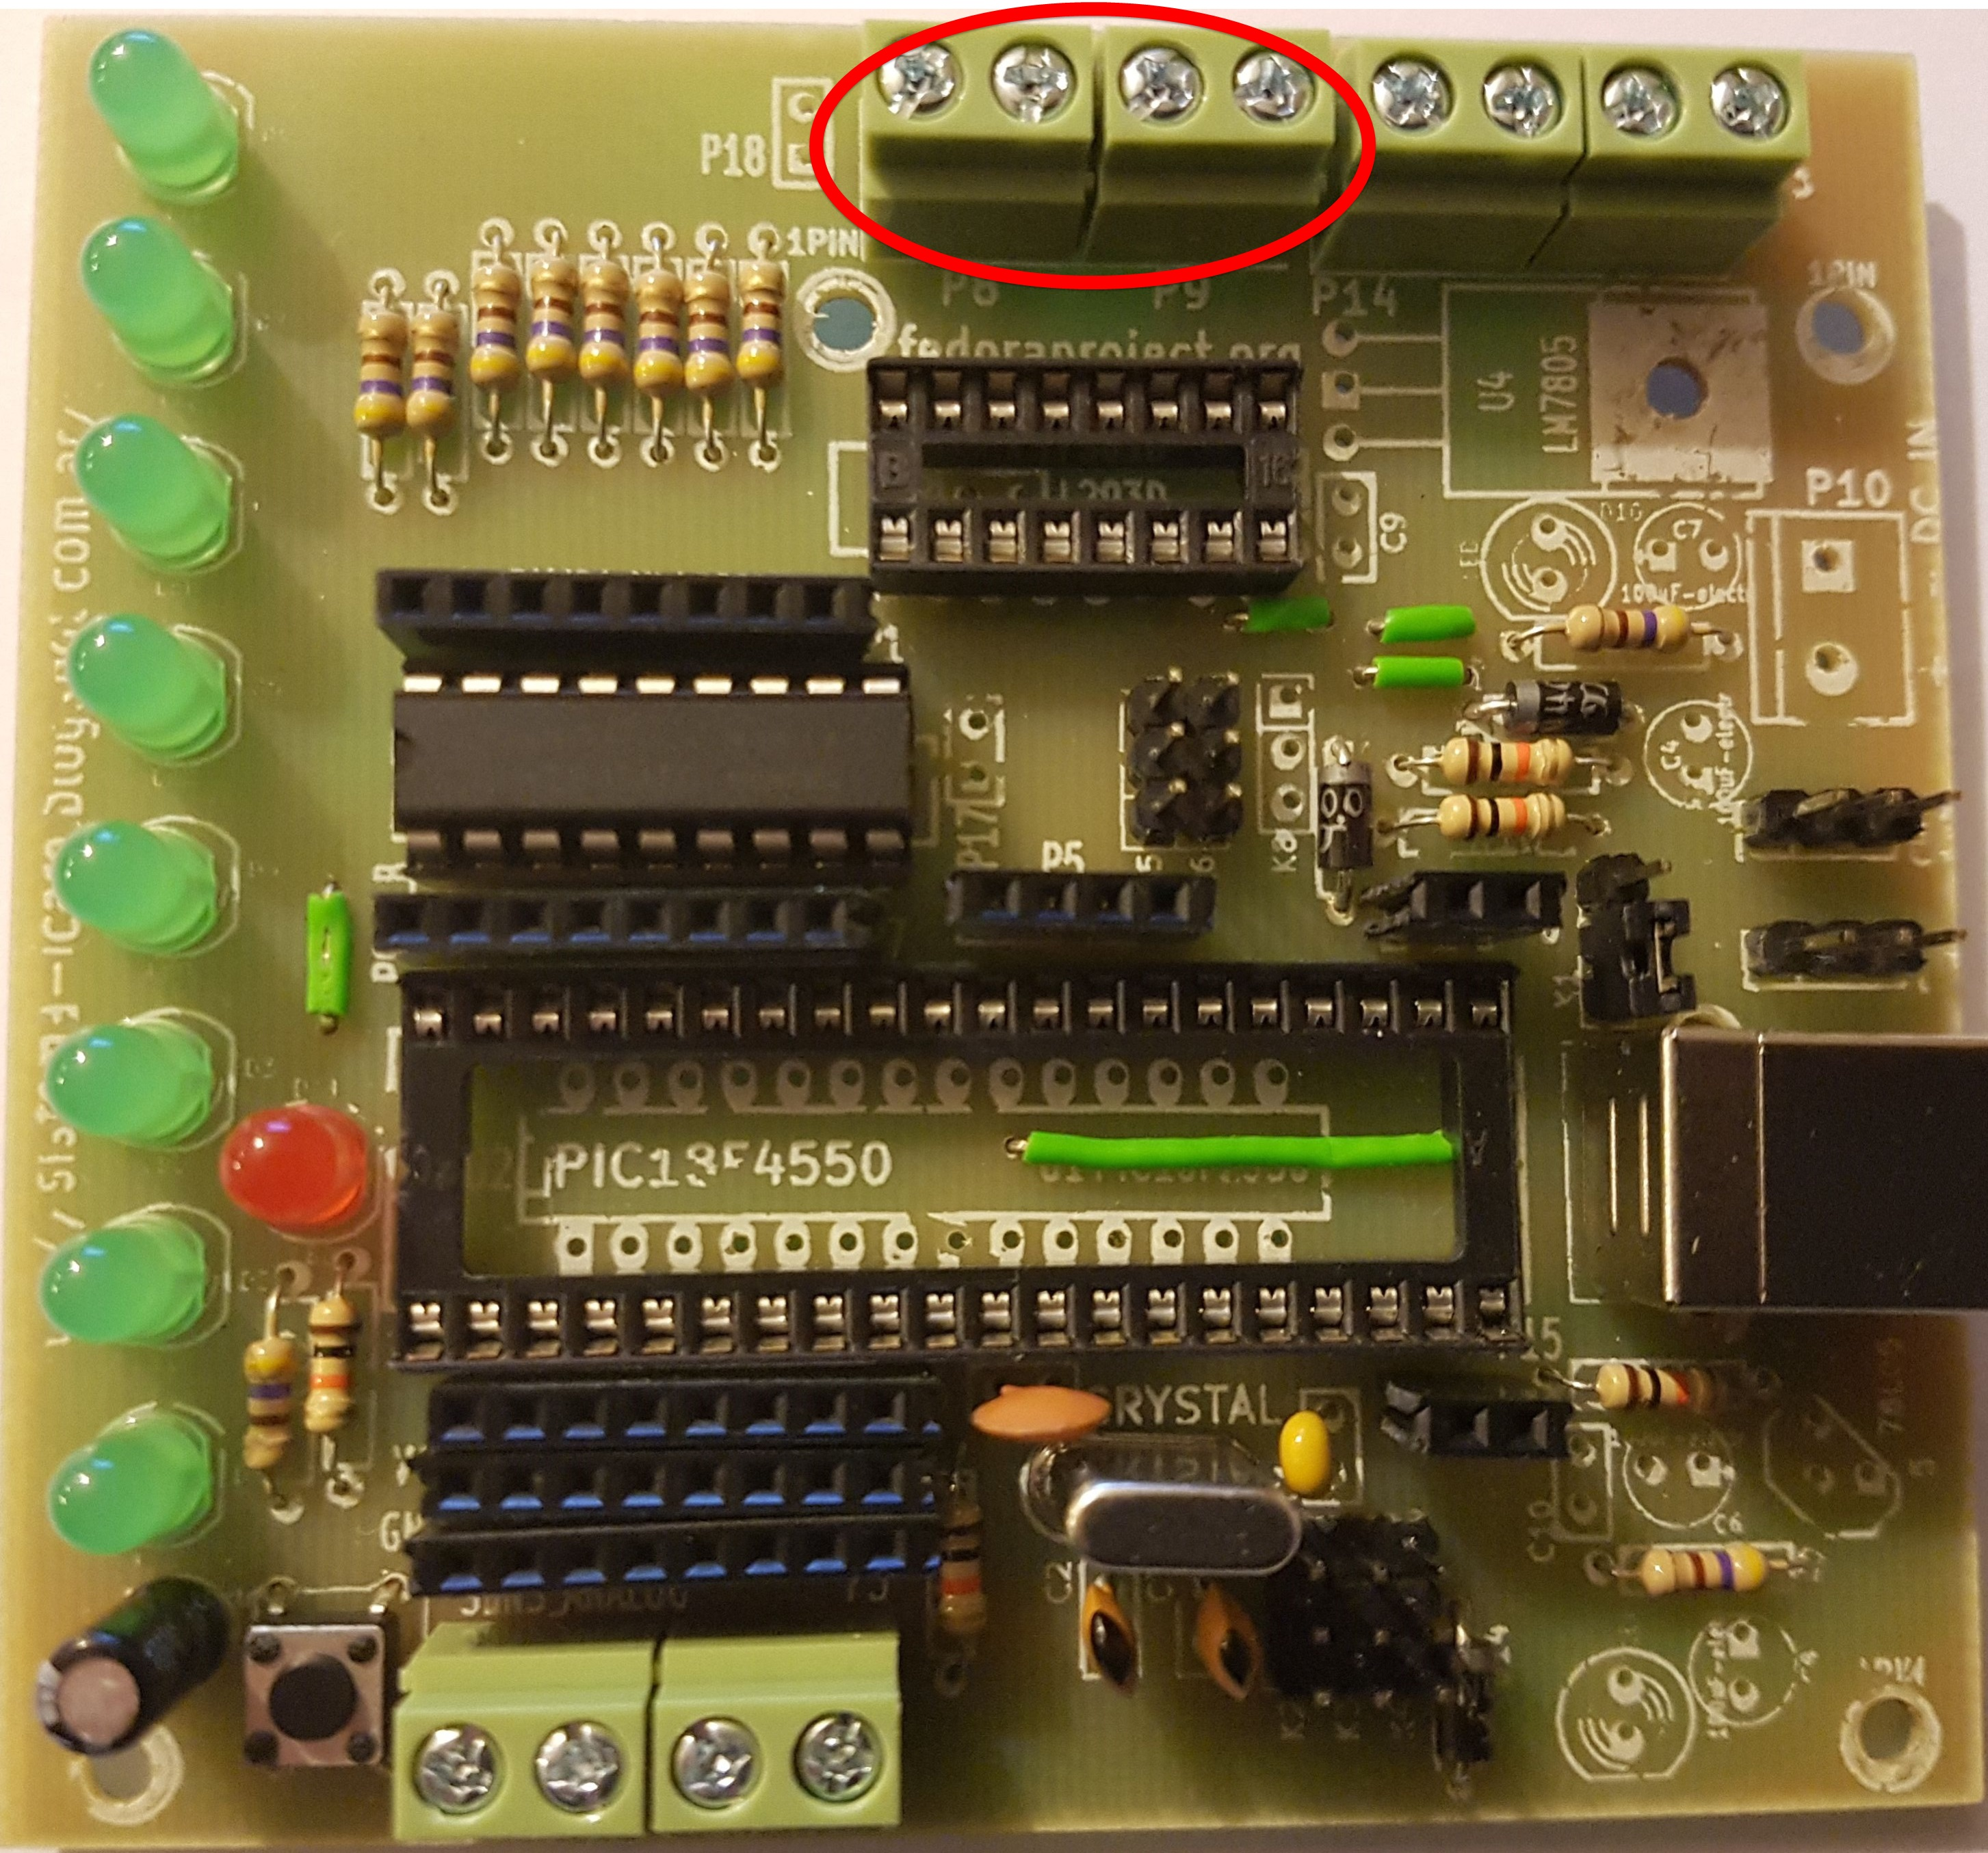
\includegraphics[width=0.8\linewidth]{Modulo_5/M5_4}
	\caption{Módulo 5 - Paso 4}
	\label{fig:M5_4}
\end{figure}

\newpage

\section{Paso 5:}

Instalar puente H L293D en U3

\begin{figure}[h]
	\centering
	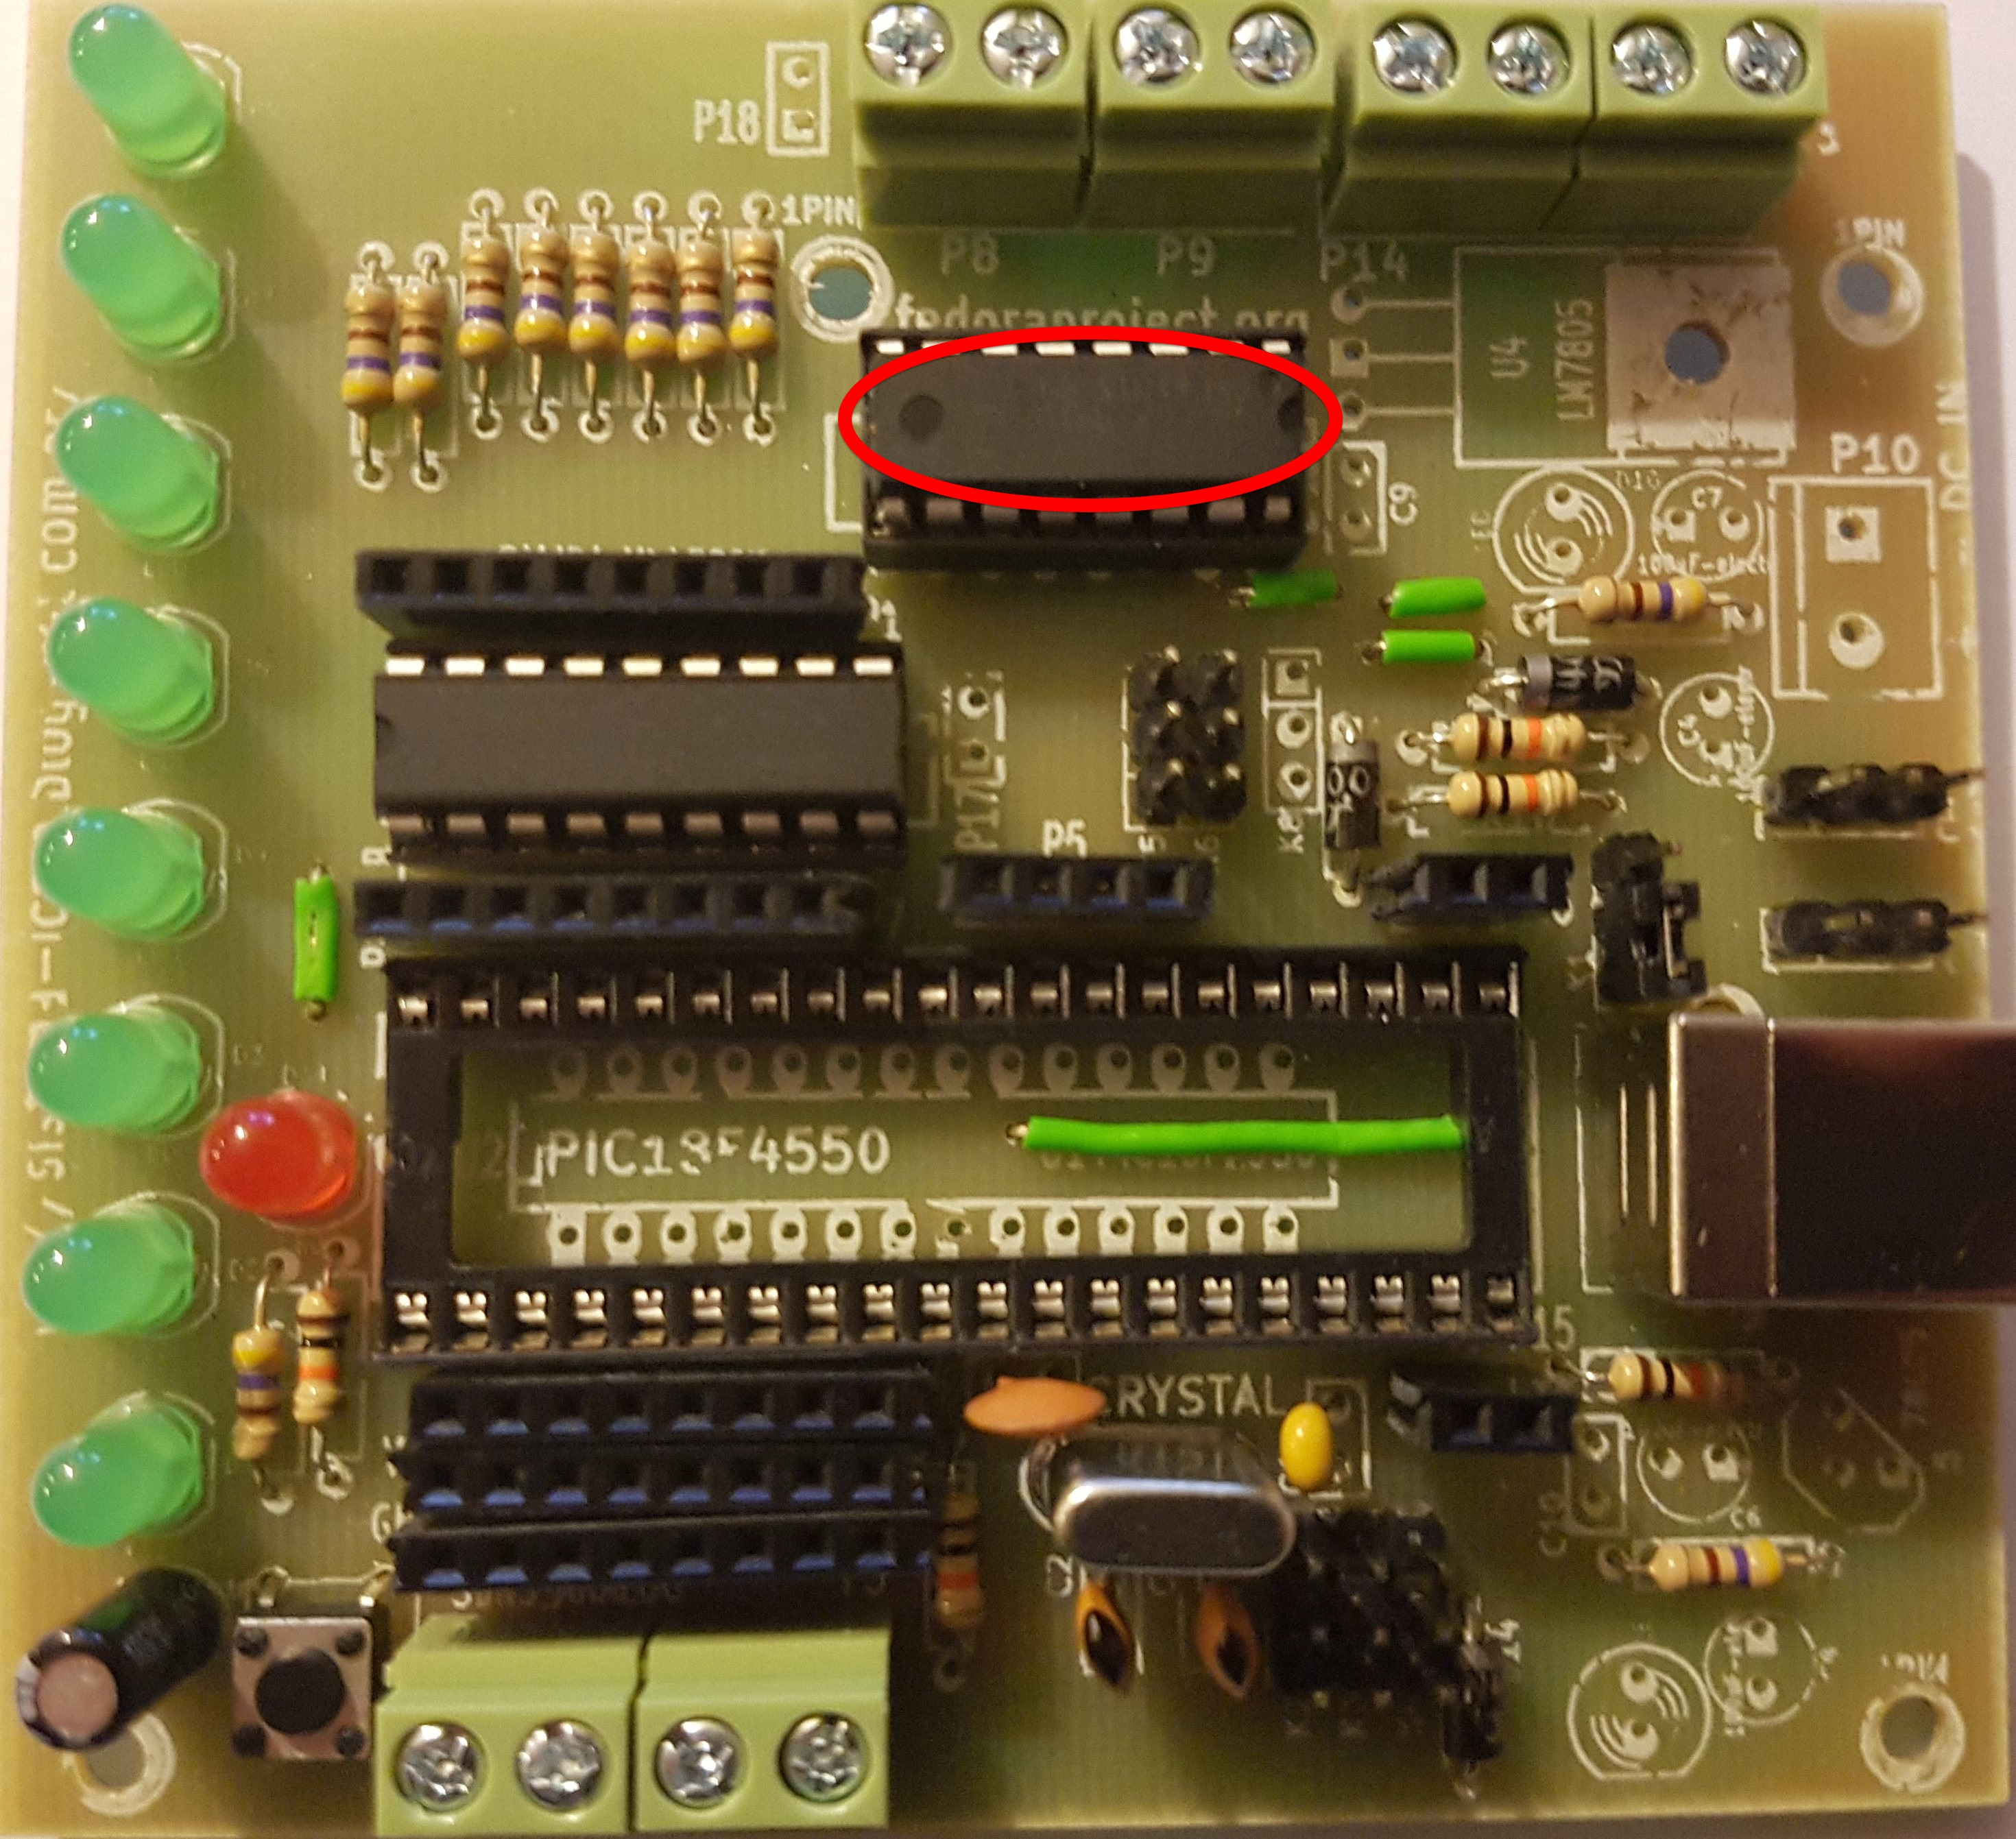
\includegraphics[width=0.8\linewidth]{Modulo_5/M5_5}
	\caption{Módulo 5 - Paso 5}
	\label{fig:M5_5}
\end{figure}